%!TEX root = Thesis.tex
\chapter{Concept}
     The chapter poses and describes a concept of a user-friendly generic frontend for exploring sensor data, 
     through designing a software architecture and a mockup of a web-based user interface that in the same time controlled and provisioned by end users request. The concept is developed based on the analysis of the current state of the art, up-to-date technologies and requirements formulated in chapter 2. 
     \newline
     Section 4.1 begins this chapter with software architecture according to 3-tier architecture, which consists client tier, application tier and data tier. Next sections presents detailed descriptions of every module, responsible for providing component functionality of every tier. Summary of this chapter underlines responsibility and requirements to every part of system infrastructure, such that prototype can be realized and implemented accordingly.


\section{3-tier Architecture}
  Since the concept of a generic frontend should be scalable and easy integrated to any kind of backend, become necessary to determine software architecture according to a 3-tier architecture, in which presentation, application processing, and data management functions are logically separated. Multitier architecture provides to developer abstract structure of every module and gives a possibility to define in which module of system developer is interested in. Also it describes how different parts of frontend interconnected with each other and what are extensions and integration's points for backend.

  Figure 4.1 shows concept infrastructure:
  \begin{itemize}
  \item \textbf{Client Tier:} web-based GUI
  \item \textbf{Application Tier:} application logic, interface of collaboration between tiers, backend integration point
  \item \textbf{Data Tier:} data from different types of sensors
  \end{itemize} 
  \begin{figure}[!ht]
  \centering
  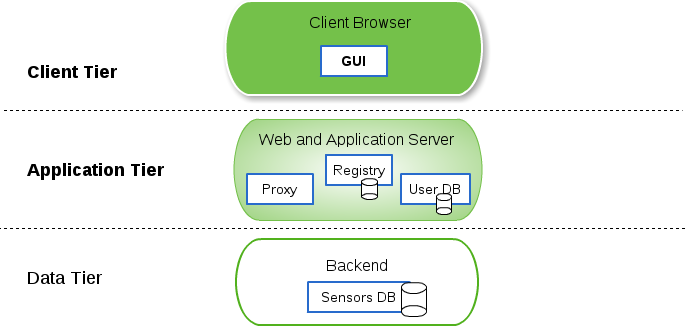
\includegraphics[scale=0.7]{images/3tier.png}   
  \caption[3-tier Architecture]{3-tier Architecture}
  \label{img:3-tier Architecture}                           
  \end{figure}

  \emph{Client Tier} hosts the presentation layer components. The main function of the interface is to translate tasks and results to graphical user interface that can be easily understandable and explorable from any kind of device. That satisfy requirements of the usability(section 3.4).
  \newline
  \emph{Application Tier} includes business logic, logic tier and data access tier. It controls an application's functionality by performing detailed processing, transformation of one type data to each other, defines an interface of interconnection between client tier and data tier. Besides possessing application logic between two another tiers of infrastructure, this tier also consists integration point for backend systems.
  \newline
  \emph{Data Tier} consists source of data that have to be retrieved by application tier to a client tier, by request from a user. This tier keeps data neutral and independent from application server or business logic. Giving data its own tier also improves scalability and loose coupling. 
  
   The three tiers architecture may seem similar to the model-view-controller (MVC) concept. However, topologically they are different. A fundamental rule in a three tier architecture is the client tier never communicates directly with the data tier; in a three-tier model all communication must pass through the middle tier. Conceptually the three-tier architecture is linear. However, the MVC architecture is triangular: the view sends updates to the controller, the controller updates the model, and the view gets updated directly from the model.
   \newline
    From a historical perspective the three-tier architecture concept emerged in the 1990s from observations of distributed systems\cite{wiki:3tier}(e.g., web applications) where the client, middleware and data tiers ran on physically separate platforms. Today, MVC and similar model-view-presenter (MVP) are Separation of Concerns design patterns that apply exclusively to the presentation layer of a larger system. In simple scenarios MVC may represent the primary design of a system, reaching directly into the database; however, in most scenarios the Controller and Model in MVC have a loose dependency on either a Service or Data layer/tier. Thus, to ensure highly adaptive GUI independently from data that have to be retrieved MVC pattern come into a picture. As a part of frontend logic it will be described in section 4.3.

  The next section gives a detailed explanation about structure modules in every tier respectively to 3-tier architecture.

\section{Client Tier}
  The client tier or another name is presentation tier is a layer which user can access directly such as a web page by using browser. It is the first that user see and comprised of widgets structured according to the responsive layout. This tier consists GUI by using which, user can communicate with sensor in a user-friendly way that is presented on the Figure 4.2. From a developer prospect of view, client tier gives an overview of a design layout, consists basic information about system architecture, provides technical details of a system such as: end-points configuration, API documentation or get sample applications. It is made in such a way, that by using only graphical interface, developer can retrieve on it personal data sources. Also Client Tier responsible for adaptation to any kind of mobile or desktop devices that can be used by user. Therefore as a cross-platform approach was chosen web-based solution, where all communication flows through the browser. 

    \begin{figure}[!ht]
    \centering
    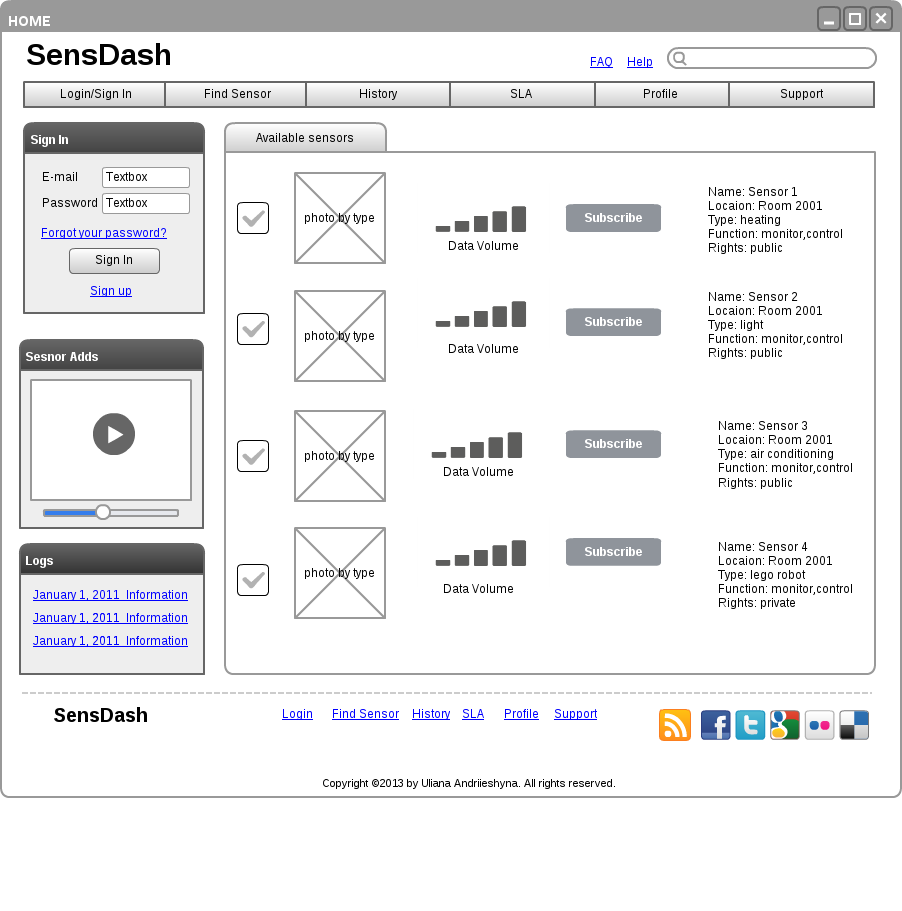
\includegraphics[scale=0.5]{images/Mockup.png}   
    \caption[GUI Mockup]{GUI Mockup}
    \label{img:GUI Mockup}                           
    \end{figure}

    Figure 4.2 presents simple content layout that have to be presented on a web-page in order to satisfy all possible user requirements. It consists:
      \begin{itemize}
      \item Main four tabs: sensors list consists a list of all available sensors; subscriptions - show all data sources to which user subscribed; favorites tab saves favorite data sources among already subscribed and settings tab gives a possibility to user, to manage own account settings and also add new sensors through the defined channel.
      \item Log in form with user name and password fields. After user logged in, the system defines his/her rights and applies visibility rules according to credentials. Independently from user rights, a user can explore description of every data retrieved by system, but only after subscription to a data sensor become possible to get streaming data, provided by sensor. User that have an admin rights receives an opportunity to control and manipulate sensors. Normal user without privileges, receives an opportunity to get statistic and information from sensors and to manipulate his/her own account data.
      \item Sensor icon defines what is the current type of sensor, e.g. light, temperature, heating, robot lego, etc. It helps user easily, even in seconds, understand and catch what is the main function of a sensor in the list, especially if among icon he/she has already used some sensors and famous producers of data.
      \item Availability or unavailability to see alive statistics. User can subscribe only to the available services. If some services become unavailable it will be automatically marked as inactive and after refreshing will be deleted from the list of available sensors. If user has already subscribed to any sensor, this sensor automatically added to a list/tab of subscriptions made by user. Also user has a possibility to define sequence order in which sensor information have to be displayed. It is done by using "favorite" label/tab. It helps user in a fast way receive information from a sensor.
      \item Data Volume icon shows what is the average data stream volume needed to retrieve sensor data(Kb/s). User can self-define how possible to get such type of streaming data according to his/her available Internet connection. Ideally, the dashboard should automatically adapt quality of streaming data to necessary and possible bandwidth of available connection(Wi-Fi, 3G, GPRS), such that it will not disturb user and other application on a mobile device.
      \item Description and preview. To give a user full information about sensed data and to help recognize how useful will be to make a subscription, the best is give a preview or examples of data. It's not only description but also real graphics, real examples of video or audio, images etc.
      \item Access and providers. Data can be private or public. If public, user don't have to accept any SLA to get real data from a sensor. But for private data very important to accept SLA between subscriber and provider, before user will get any real data.
      \item Search panel. Have to be done by filtering available sensors only based on information available for Frontend. Without any queries to Backend and waiting for answer.
      \end{itemize}

    The common use case shown on Figure 4.3. User can use any type of mobile device and his favorite browser to receive information from data sources(sensors) by using web-page as a dashboard. Once a user log in to the dashboard, he/she can explore all available sensors around him. If he/she already has used this dashboard at another location and subscribed to some sensors, it will be automatically available in another tab named subscriptions. 

        \begin{figure}[!ht]
        \centering
        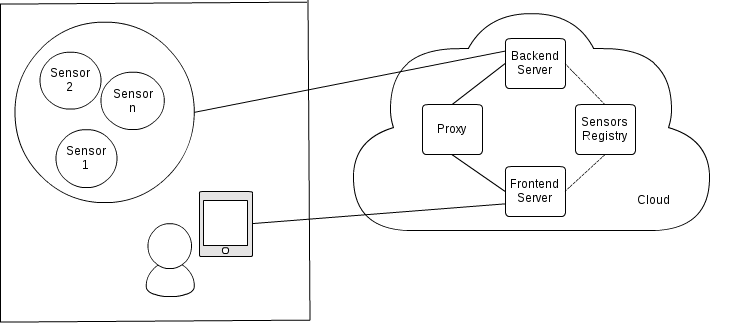
\includegraphics[scale=0.6]{images/User_Case.png}   
        \caption[Use Case]{Use Case}
        \label{img:structure}                           
        \end{figure}

\section{Application Tier}
  This layer coordinates the application, processes commands, makes logical decisions and evaluations, and performs calculations. It also moves and processes data between the two surrounding layers.

  Application tier consists all logical modules as: Web server, Sensor registry, Data Hub and Web-based Frontend. All these modules connects to each other as shown on the Figure 4.4. 
    \begin{figure}[!ht]
    \centering
    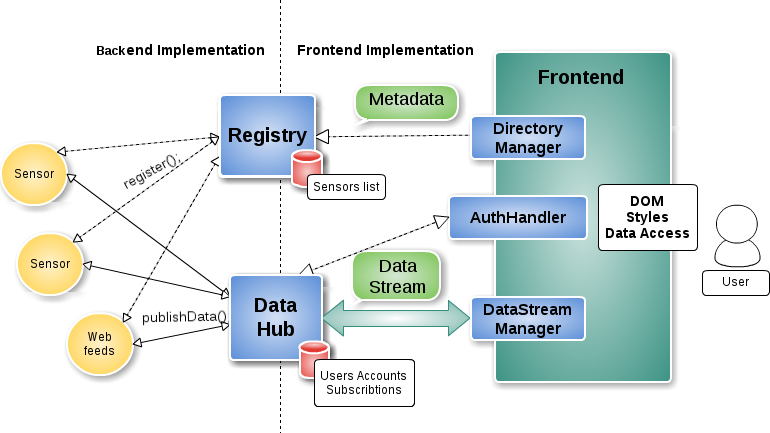
\includegraphics[scale=0.6]{images/Structure.png}   
    \caption[System Architecture]{System Architecture}
    \label{img:structure}                           
    \end{figure}

    System Architecture splitted to a backend and frontend implementation, that gives an overview how these two part interconnected. Also on the Figure 4.4 presents a end-user, which doesn't know anything about implementation behind the scenes. Registry and Data Hub defined and standardized by frontend in order to provide as much as possible common interface for collaboration between backend and frontend. 

  \subsection{Sensors Registry}
    First of all the Sensors Registry is a module responsible for storing an info about available sensors registered in the network in order to provide information for a user. Frontend gets info from Registry about registered sensors and their availability. By using simple Web API, so that any Registry that implements suggested API and returns valid JSON, which consists such info as: id of sensor, description, availability(true or false), access(private or public), provider of sensed data, SLA, necessary bandwidth for retrieving data, title and type. By using Web API, the concept provides a possibility to dynamically connect and disconnect different Registries, that are required in a different context of usage. 
    \newline
    Before publishing data to Registry, a data publisher must first register the sensor by providing its static description. This meta data describes sensor name, sensing type, availability, data type, access type, provider name and further details, and also if possible some real examples of data or preview possibility, as well as a free text description of the sensors, and is used in searching sensors for a given user query.
    \newline
    Such structure helps system to structure sensors according to the type, as a result to automatically generate the graphical container for it. Based on standard description, rendering of the sensor data in the client tier become essential part, because it simplifies the way of sensors integration. 

    And secondary, the Registry, provides simple interface standard in JSON format to encode these properties that can be simply transferred by using Web API approach. Thus, it is much simpler and light-weighted than XML. And separate metadata of a sensor from a real data. 

  \subsection{Data Hub}
    Since Sensors Registry responsible for collecting metadata of sensors, Data Hub is responsible for mapping interface of particular sensor data stream into a format supported by frontend and delivered through the common universal protocol. It means that Data hub has to satisfy next requirements:

    \begin{itemize}
    \item be aware of metadata provided by Registry to frontend
    \item bind metadata from registry and user choice
    \item get and parse sensor streaming data and reconvert it to the type supported by universal protocol
    \item implement universal protocol to provide exchange message with a server in order to make possible retrieve streaming data from sensor
    \item store history of a data sources
    \end{itemize}

    \subsubsection{Authentication Handler}
    Authentication Handler responsible for registering user in system, providing User ID and define user role. After a user gets necessary ID and confirm his/her personality by using password and name, system automatically applies visibility rules. After a user verifies and confirms credentials, it becomes possible to bind user id with personal preferences. Such preferences can be: user subscriptions, favorites, social sharing and even cookies. Since all these data have to be loosely coupled from backend, and web-based application has no access to internal storage of portable device, this problem solved enhancing functionality of XMPP protocol and using namespace approach of XMPP server storage.

    \textbf{Backend entry point}
    Data Hub and Sensor Registry are two modules that have been standardized by frontend and have to be fully implemented on a backend side. Since both of this parts support common standards such as Web API, HTTP GET, AJAX, JSON file format, it makes easily possible to implement it inside any backend system.

  \subsection{Web-based Frontend}
    \subsubsection{Web server}
      The primary function of a web server is to deliver web pages to clients. The communication between client and server takes place using the Hypertext Transfer Protocol (HTTP). Pages delivered are most frequently HTML documents, which may include images, style sheets and scripts in addition to text content. 
      \newline 
      In proposed concept Web server is responsible for robust and efficient serving of static files. The goal is to exclude dependencies on concrete backend platforms or frameworks and to provide generic frontend as easily plugable component. Such a common and simplified design decision makes possible to extend and scale every part of distributed system independently. Specific operation logic like authentication of user, registration of sensors and users are delegated to external components such as Registry, Data Hub and Authentication Nadler, these external components can be interchanged without dependency to the system itself.

    \subsubsection{Interfaces}
      On the Figure 4.4 from a frontend prospect of view exist 3 communication channels: 
      \begin{itemize}
      \item Registry to Directory Manager (one-way connection)
      \item Data Hub to/from DataStream Handler (asynchronous duplex connection) 
      \item Data Hub to/from AuthHandler (synchronous duplex connection) 
      \end{itemize}

      \emph{Registry to Directory Manager Interface}
      \newline
      According to Web API and simple structure of a registry data, communication between these two modules have to be done by using HTTP GET request and JSON format, retrieved from Registry. It is one-way connection, because frontend needs only get metadata from Sensors Registry and all changes that occurs on a web page end through interface between Data Hub and DataStream Handler. Such structure provides possibility independently integrate new Sensors Registry.

      \emph{Data Hub to/from Directory Manager Interface/AuthHandler}
      \newline
      Communication between Data Hub and another 2 modules: Directory Manager Interface and AuthHandler, have to be supported through the one common universal interface. This interface have to satisfy next requirements:
      \begin{itemize}
      \item have a public license
      \item handle Web API requests
      \item support service-user n:n connections
      \item support different types of data sended through the one channel, message differentiation
      \item keep connection alive(stateful, through the TCP connection)
      \item simplicity of enhancement and customization
      \end{itemize}

      Three inetfaces have to work with data sources in the way that shown on Figure 4.4

      \begin{figure}[!ht]
      \centering
      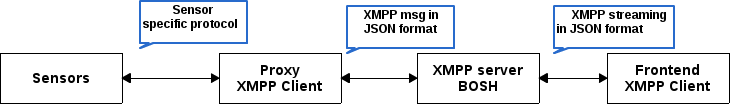
\includegraphics[scale=0.6]{images/Protocol_flow.png}   
      \caption[Protocol flow]{Protocol flow}
      \label{img:protocol}                           
      \end{figure}
      Such a structure decouple sensors specific interface and interface between frontend and backend. In such a way, any sensor can be added and retrieved by frontend. 
    
      The web browser is probably the most deployed and most used application platform that has ever existed. Web browsers exist on every kind of computer and even many mobile phones, and more importantly, the users of these devices tend to be very familiar with the browser and web applications. As more and more sophistication has been demanded of web applications, new technologies and abstractions have been created to evolve the platform. XMPP brings yet another new set of technologies and abstractions, but with it comes enormous potential for real-time, interactive, and collaborative applications. The rise of the social Web has given rise to social applications, and if developers want to take more steps toward connecting the human race, technologies like XMPP will help them do it. For XMPP developers, targeting the web browser as a platform makes enormous sense.

      In order to satisfy all aforementioned requirements, nowadays exist two main protocols: \emph{XMPP\cite{XMPPbook}}:a protocol best for connecting devices to people, a special case of the device-to-server pattern, since people are connected to the servers and \emph{MQTT\footnote{MQ Telemetry Transport,\url{http://mqtt.org/}}}: a protocol for collecting device data and communicating it to servers. Based on their functionality and specification can be managed questions of authentification, registration and user preferences storage.

      \textbf{MQTT}
      \newline
      the Message Queue Telemetry Transport, targets device data collection (Fig. 4.6). As its name states, its main purpose is telemetry, or remote monitoring. Its goal is to collect data from many devices and transport that data to the IT infrastructure. It targets large networks of small devices that need to be monitored or controlled from the cloud.
      \begin{figure}[!ht]
      \centering
      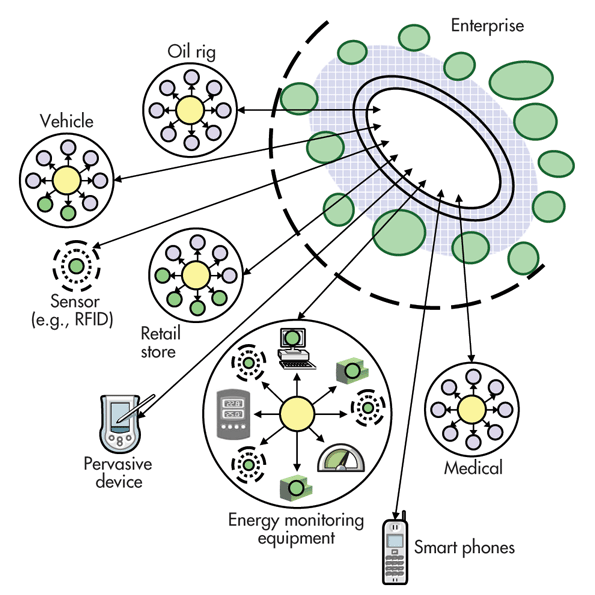
\includegraphics[scale=0.6]{images/MQTT.png}   
      \caption[Message Queue Telemetry Transport]{Message Queue Telemetry Transport}
      \label{img:MQTT}                           
      \end{figure}
      MQTT makes little attempt to enable device-to-device transfer, nor to "fan out" the data to many recipients. Since it has a clear, compelling single application, MQTT is simple, offering few control options. It also doesn’t need to be particularly fast. In this context, "real time" is typically measured in seconds.

      A hub-and-spoke architecture is natural for MQTT. All the devices connect to a data concentrator server. So the protocol works on top of TCP, which provides a simple, reliable stream. Since the IT infrastructure uses the data, the entire system is designed to easily transport data into enterprise technologies like ActiveMQ and enterprise service buses (ESBs).

      MQTT enables applications like monitoring a huge oil pipeline for leaks or vandalism. Those thousands of sensors must be concentrated into a single location for analysis. When the system finds a problem, it can take action to correct that problem. Other applications for MQTT include power usage monitoring, lighting control, and even intelligent gardening. They share a need for collecting data from many sources and making it available to the IT infrastructure.

     \textbf{XMPP}
      \newline 
      XMPP was originally called "Jabber". It was developed for instant messaging (IM) to connect people to other people via text messages (Fig. 4.7). XMPP stands for Extensible Messaging and Presence Protocol. Again, the name belies the targeted use: presence, meaning people are intimately involved.
      \begin{figure}[!ht]
      \centering
      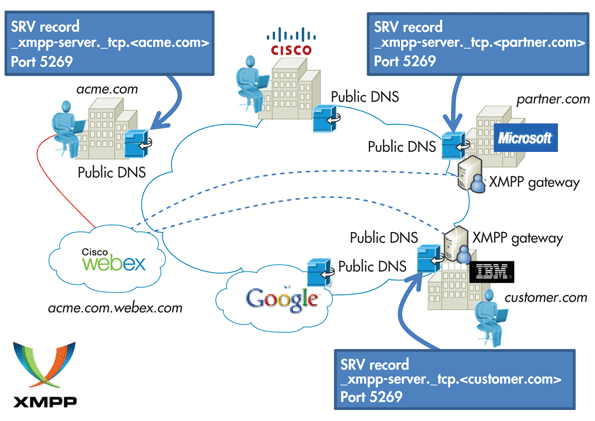
\includegraphics[scale=0.7]{images/XMPP.png}   
      \caption[The Extensible Messaging and Presence Protocol (XMPP)]{The Extensible Messaging and Presence Protocol (XMPP)\footnote{IoT, \url{http://electronicdesign.com/embedded/understanding-protocols-behind-internet-things}}}
      \label{img:XMPP}                           
      \end{figure}
      XMPP uses the XML text format as its native type, making person-to-person communications natural. Like MQTT, it runs over TCP, or perhaps over HTTP on top of TCP. Its key strength is a name@domain.com addressing scheme that helps connect the needles in the huge Internet haystack.

      In the IoT context, XMPP offers an easy way to address a device. This is especially handy if that data is going between distant, mostly unrelated points, just like the person-to-person case. It’s not designed to be fast. In fact, most implementations use polling, or checking for updates only on demand. A protocol called BOSH (directional streams over Synchronous HTTP) lets severs push messages. But "real time" to XMPP is on human scales, measured in seconds. Its strengths in addressing, security, and scalability make it ideal for consumer-oriented IoT applications.

      XMPP powers a wide range of applications including instant messaging, multi-user chat, voice and video conferencing, collaborative spaces, real-time gaming, data synchronization, and even search. Although XMPP started its life as an open, standardized alternative to proprietary instant messaging systems like ICQ and AOL Instant Messenger, it has matured into an extremely robust protocol for all kinds of exciting creations.

      After a sort introduction become clear that XMPP fully satisfy all requirements in order to be used in concept of generic frontend. So the interface \emph{Data Hub to/from Directory Manager Interface/AuthHandler} provided by using XMPP.
      \newline
      The core of XMPP is the exchange of small, structured chunks of information. Like HTTP, XMPP is a client-server protocol, but it differs from HTTP by allowing either side to send data to the other asynchronously. XMPP connections are long lived, and data is pushed instead of pulled. Because of XMPP’s differences, it provides an excellent companion protocol to HTTP. XMPP-powered web applications are to AJAX what AJAX was to the static web site; they are the next level of interactivity and dynamism. Where JavaScript and dynamic HTML have brought desktop application features to the web browser, XMPP brings new communications possibilities to the Web. XMPP has many common social web features built in, due to its instant messaging heritage. Contact lists and subscriptions create social graphs, presence updates help users keep track of who is doing what, and private messaging makes communication among users trivial. XMPP also has nearly 300 extensions, providing a broad and useful range of tools on which to build sophisticated applications. 
      \newline
      XMPP, like all protocols, defines a format for moving data between two or more communicating entities. In XMPP’s case, the entities are normally a client and a server, although it also allows for peer-to-peer communication between two servers or two clients. Many XMPP servers exist on the Internet, accessible to all, and form a federated network of interconnected systems. Data exchanged over XMPP is in XML, giving the communication a rich, extensible structure. Many modern protocols forgo the bandwidth savings of a binary encoding for the more practical feature of being human readable and therefore easily debugged. XMPP’s choice to piggyback on XML means that it can take advantage of the large amount of knowledge and supporting software for dealing with XML. One major feature XMPP gets by using XML is XML’s insensibility. It is extremely easy to add new features to the protocol that are both backward and forward compatible. This extensibility is put to great use in the more than 200 protocol extensions registered with the XMPP Standards Foundation and has provided developers with a rich and practically unlimited set of tools. XML is known primarily as a document format, but in XMPP, XML data is organized as a pair of streams, one stream for each direction of communication. Each XML stream consists of an opening element, followed by XMPP stanzas and other top-level elements, and then a closing element. Each XMPP stanza is a first-level child element of the stream with all its descendant elements and attributes. At the end of an XMPP connection, the two streams form a pair of valid XML documents.
      The Extensible Messaging and Presence Protocol (XMPP) is the IETF’s formalization of the base XML streaming protocols for instant messaging and presence developed within the Jabber community starting in 1999\cite{xmpp}.

      \textbf{Pushing Data}

      HTTP clients can only request data from a server. Unless the server is responding to a client request,
      it cannot send data to the client. XMPP connections, on the other hand, are bidirectional. Either party
      can send data to the other at any time, as long as the connection is open.
      This ability to push data greatly expands the possibilities for web applications and protocol design.
      Instead of inefficient polling for updates, applications can instead receive notifications when new
      information is available. Not only does this result in many fewer requests, it also makes the latency
      between the time new information is available and the time the client is aware of this information
      nearly zero.

      \textbf{Pleasing Firewalls}

      Some web applications support the use of HTTP callbacks, where the web server makes requests to
      another HTTP server in order to send data. This would be a handy feature to push data if it weren’t
      for firewalls, network address translation (NAT), and other realities of the Internet. In practice it is
      very hard to enable arbitrary connections to clients from the outside world.
      XMPP connections are firewall and NAT friendly because the client initiates the connection on
      which server-to-client communication takes place. Once a connection is established, the server can
      push all the data it needs to the client, just as it can in the response to an HTTP request.

      \textbf{Improving Security}

      XMPP is built on top of TLS and SASL technologies, which provide robust encryption and security
      for XMPP connections. Though HTTP uses SSL, the HTTP authentication mechanisms did not see
      much implementation or use by developers. Instead, the Web is full of sites that have implemented
      their own authentication schemes, often badly.

      \textbf{Statefulness}

      HTTP is a stateless protocol; XMPP is stateful. Stateless protocols are easier to scale because each
      server does not need to know the entire state in order to serve a request. This drawback of XMPP
      is less onerous in practice because most non-trivial web applications make extensive use of cookies,
      backend databases, and many other forms of stored state.
      Many of the same tools used to scale HTTP-based applications can also be used to scale XMPP-based
      ones, although the number and diversity of such tools is more limited, due to XMPP’s younger age and
      lesser popularity.

    \begin{itemize}
      \item \emph{Decentralization}
        The architecture of the XMPP network is similar to email; anyone can run their own XMPP server and there is no central master server.
     \item \emph{Open standards}
        The Internet Engineering Task Force has formalized XMPP as an approved instant messaging and presence technology under the name of XMPP (the latest specifications are RFC 6120 and RFC 6121). No royalties are required to implement support of these specifications and their development is not tied to a single vendor.
      \item \emph{History}
        XMPP technologies have been in use since 1999. Multiple implementations of the XMPP standards exist for clients, servers, components, and code libraries.
      \item \emph{Security}
        XMPP servers can be isolated from the public XMPP network (e.g., on a company intranet), and strong security (via SASL and TLS) has been built into the core XMPP specifications.
      \item \emph{Flexibility}
        Custom functionality can be built on top of XMPP; to maintain interoperability, common extensions are managed by the XMPP Standards Foundation. XMPP applications beyond IM include group chat, network management, content syndication, collaboration tools, file sharing, gaming, remote systems control and monitoring, geolocation, middleware and cloud computing, VoIP and Identity services.
      \end{itemize}

      \begin{figure}[!ht]
      \centering
      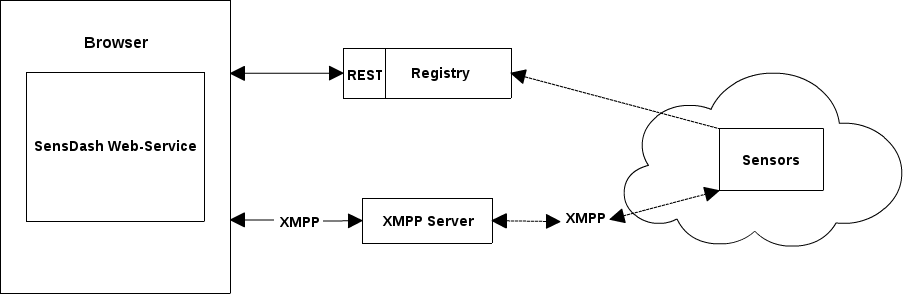
\includegraphics[scale=0.5]{images/Interface.png}   
      \caption[Interface]{Interface}
      \label{img:interfaces}                           
      \end{figure}

      The XMPP network uses a client–server architecture (clients do not talk directly to one another). However, it is decentralized by design, there is no central authoritative server, as there is with services such as AOL Instant Messenger or Windows Live Messenger. Some confusion often arises on this point as there is a public XMPP server being run at jabber.org, to which a large number of users subscribe. However, anyone may run their own XMPP server on their own domain.
      Every user on the network has a unique Jabber ID (usually abbreviated as JID). To avoid requiring a central server to maintain a list of IDs, the JID is structured like an email address with a username and a domain name (or IP address) for the server where that user resides, separated by an at sign (@), such as username@example.com.

  \subsubsection{JavaScript MVC}
    JavaScript has become one of the most popular programming languages on the web, when the usage of Ajax came to light and professional programmers gave importance to the responsiveness of the page. But now the language has become more popular than ever as the User Experience has become the key part of web development. Accessing web is not limited to browsers alone – there are lot many devices with varying screen sizes accessing the same content. With the rise of HTML5 and CSS3 the web will become more adaptive and responsive than ever and JavaScript plays a major role in it. It has also gained popularity in the server side programming which is made possible by NodeJS framework.

    Increase in usage of JavaScript in modern applications demand developers to write maintainable code, separate concerns and improve testability. JavaScript is a "class" less language and it was not designed to support Object Oriented Programming. There are some DOM manipulation libraries like jQuery which simplifies client side scripting of HTML, they actually do not solve the problem of effectively handling separation of concerns. The problem with this is that it doesn’t take long to get lost in a nested pile of jQuery callbacks and DOM elements without any real structure in place for applications. Source code that has a complex and tangled control structure, especially one using many GOTOs, exceptions, threads, or other "unstructured" branching constructs can lead to become a bottleneck. 
     \begin{figure}[!ht]
     \centering
     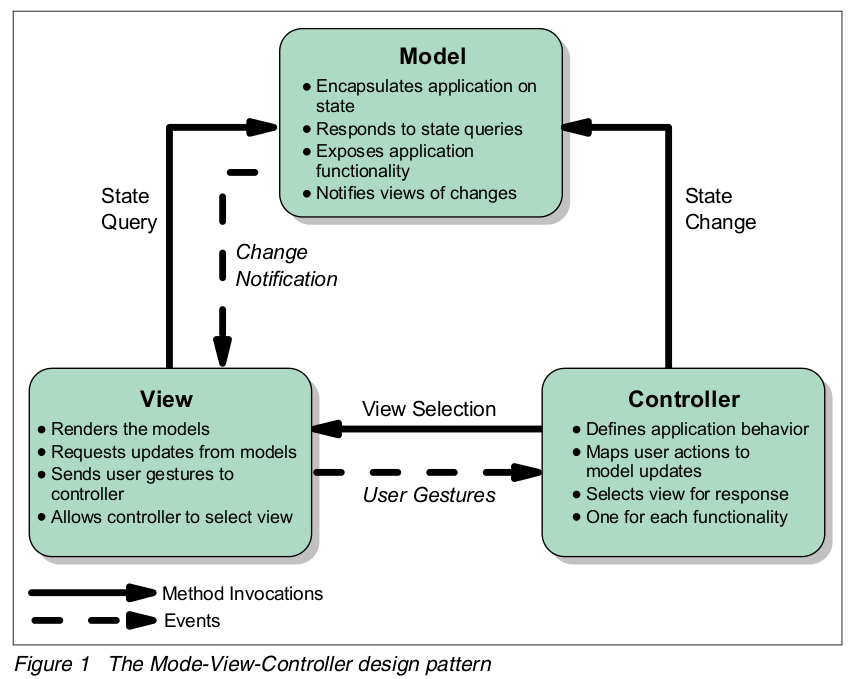
\includegraphics[scale=0.5]{images/MVCPattern.png}   
     \caption[MVC Pattern]{MVC Pattern\footnotetext{Image taken from, \url{blog.csdn.net/cain/article/details/6617173}}}
     \label{img:MVCPattern}                           
     \end{figure}

    In the design shown on the Figure 4.9, takes place common Model-View-Controller pattern. Where a Model represents the application object that implements the application data and business logic. The View is responsible for formatting the application results and dynamic page construction. The Controller is responsible for receiving the client request, invoking the appropriate business logic, and based on the results, selecting the appropriate view to be presented to the user. The Model represents enterprise data and the business rules that govern access to and updates to this data. Often the Model serves as a software approximation to a real-world process, so simple real-world modeling techniques apply when defining the Model. A View renders the contents of a Model. It accesses enterprise data through the Model and specifies how that data should be presented. It is the View's responsibility to maintain consistency in its presentation when the Model changes. This can be achieved by using a push Model, where the View registers itself with the Model for change notifications, or a pull Model, where the View is responsible for calling the Model when it needs to retrieve the most current data. A Controller translates interactions with the View into actions to be performed by the Model. In a stand-alone GUI client, user interactions could be button clicks or menu selections, whereas in a Web application, they appear as GET request. The actions performed by the Model include activating business processes or changing the state of the Model. Based on the user interactions and the outcome of the Model actions, the Controller responds by selecting an appropriate View. 

  Though all the frameworks out there somewhat tries to be MVC but they do not necessarily follow the pattern strictly. The idea of all the patterns is to separate Model, View and Logic that hooks the two behind which is the controller for the best separate of concerns. On the other side we do have other libraries which implement Model-View-Presenter(MVP) and Model-View-ViewModel(MVVM) pattern. For this reason we will refer these frameworks as MV* implementation. So it's much more depends on framework and researched in the Chapter 5 in details.
      

\section{Data Tier}
   As was mentioned in section 4.1 Data Tier consists source of data that have to be retrieved by application tier to a client tier. Also this tier is a entry point for backend system, thus all requirements to it already described in the section 4.3. Besides aforementioned requirements, based on section 2.2, which provides widely encompassing overview of data sources, according to it made typization of data. A User, neither a developer have to be clarified with different types of data sources that cover generic frontend. According to it, data sources can be retrieved by web page as plain text, maps of value(in order to draw graph) and images.

   These three types of data changes with some time-frequency and automatically retrieved by client tier as a streaming data. So an essential part to is to determine possible characteristics of streaming data that can be retrieved by Client Tier in a lightweight scenario for mobile devices.
   \newline
    Streaming data is multimedia that is constantly received by and presented to an end-user while being delivered by a provider. Its verb form, "to stream", refers to the process of delivering media in this manner; the term refers to the delivery method of the medium rather than the medium itself. In general, media files can be delivered in one of three ways, via streaming, progressive download, or adaptive bitrate streaming.  Each has its purpose.
  \newline
    Streaming involves delivering the media to the client via a server process using specific streaming protocols (such as XMPP).  Video playing begins almost immediately, especially if the video file was encoded at a data rate similar to the effective bandwidth of the target viewer.  Streaming video is also often not cached by the client so a local copy of the video is not held in its entirety on the client machine.  While it is not impossible for an enterprising person to capture and hold a copy of the stream, it takes more effort than the casual viewer may be willing to take on.  To adapt for the slowest common denominator in regard to end-user bandwidth, streaming videos are often encoded at lower quality and data rates.
  \newline
    Progressive download simply delivers a media file via traditional web server technologies.  The file begins playing on the client as soon as enough data has been buffered to provide a smooth uninterrupted viewing experience.  Progressive downloaded files are easier to capture since an entire copy of the file is downloaded to the local device.  Also, the quality of the file can be higher simply because a user on a slower connection will just have to wait longer for the viewing to begin.
  \newline
    Adaptive bitrate streaming is a kind of best of both worlds.  As the name implies, adaptive bitrate is a streaming technology and generally requires a dedicated streaming server.  In this case, media files are transcoded into multiple bitrates with the appropriate streaming being delivered to the user based on their available bandwidth.  Adaptive streaming servers can also dynamically change the bitrate as network conditions dictate\cite{ilias2013study}.
  \newline
  This explanation shows that adaptive bitrate streaming is the most valuable and suitable for concept of a generic frontend.
  But it is necessary to go deeply in details to define limits and understanding of "good quality", "bad quality", "excellent quality".
  All three delivery methods are forms of Adaptive Bit Rate Streaming. This delivery method will have a massive impact on every aspect of Internet streaming delivery because it allows the stream to actually adapt the streaming experience to the quality of the network and the device's CPU.
  \newline
  In other words, the media stream can increase or decrease the bit rate and resolution (its quality) in real time so that it’s always streaming the best possible quality the available network connection can support. The better the network connection, the better the video image quality. The fact that the stream handles all of this complexity means the mobile video viewer doesn’t have to do anything; everything is left to the stream and the player.

  An important aspect in streaming data that some of data can be cashed on a server side, thus become possible to retrieve data after it was produced. But some streaming data consists only live data, thus there is no other options except live streaming, where the connection configuration, aliveness and quality become a key aspect. Consider absence of any concrete backend system, cashing on it's side and on frontend side can be covered in scope of this Master Thesis. As a good example of live streaming will be simulated map of values, images and text.

  \textbf{Sensor Functional Characteristics}
  \newline
  An essential part of concept to garantee reliable and secure data transportation. Thus, based on a system architecture every data source can acquire additional properties:
  \begin{itemize}
  \item reliability
  \item perfomance
  \item security
  \end{itemize}
  All these three characteristics rely on quantity of available DataHubs which includes XMPP modules and provides data streaming. Since DataHub have to provide data from sensor through XMPP connection it has to support XMPP data channel configurations and plays a role of end-point for Frontend. If sensor has 2 end-points it should be mentioned in Sensor Registries attribute, the same as type of data transfer protocol(PubSub or MUC).

  A simple sensor, with a low level of reliability, has one and only one end-point. A reliable sensor has two end-points, where is one is a primary, the other one is a backup/failover. A highly reliable sensor has three endpoints, which is guarantee data receiving in case if another end-points will failover. 

  A high-performance sensor has more than 2 end-points, out of which one is always chosen based on minimal latency message income. In case of big data transportation all data can be splitted and sended in parallel through the more than 2 end-points. 

  A secure sensor has at least two end-points, each of which carries some part of a data. Without each part become not possible to retrieve whole data at all. 

 All this characteristics have to be automatically captured by Frontend from a predefined attributes in a standard specification provided by Registry. So that developers can get to know about the expected quality of the data streams even in case some endpoints become unavailable or add new end-points. In the meanwhile, Frontend has predefined logic, which calculate numbers of related end-point for every sensor and by using graphical elements such as icons and labels, presents this information to the user.

\section{Summary}
	In this chapter, according to a 3-tier architecture, the first web-based concept for sensor streaming services is to be created. Such type of structure provides clear separation of concern between different module of concept. Client tier consists GUI description and content, Application Tier provides application logic in order to interconnect backend and Client Tier, and finally Data Tier describes typization of data in order to easily interconnect it with Application Tier and visually retrieve it by using Client Tier. To every data souce was assigned such characteristics as reliability, perfomance and level of secure information. Every characteristics rely on a number of dependent for sensor XMPP end-point.
  As a result was identified next most important modules of Application Tier: Sensors Registry, Data Hub, AuthHandler. 

  Data Hub responsibilities:
  \begin{itemize}
  \item be aware of metadata provided by Registry to frontend
  \item bind metadata from registry with user choice
  \item get and parse sensor streaming data and reconvert it to the type supported by XMPP protocol
  \item implement XMPP protocol to provide exchange message with XMPP server in order to make possible retrieve streaming data from sensor through XMPP server
  \end{itemize}
  Registry responsibilities:
  \begin{itemize}
  \item stores an info about available sensors registered in the network
  \item provides simple interface standard in JSON format
  \end{itemize}
  Web-server responsibilities:
  \begin{itemize}
  \item handles delivery to end user static structure of the web-page
  \end{itemize}
  Frontend responsibilities:
  \begin{itemize}
  \item Interconnect all modules by using appropriate interfaces: Web API for Sensors Registry and XMPP Protocol for Data Hub and AuthHandler
  \item Build a responsive and adaptable to changes GUI
  \item Scalable system structure
  \end{itemize}
    Backend responsibilities:
  \begin{itemize}
  \item Implement Data Hub interface including XMPP with required extensions
  \item Implement Sensors Registry
  \end{itemize}